

\chapter{RTL}

\section{Introduction}

So far we have used combinational logic to describe simple circuits, but at some point we need to describe more complex logic.

In order to do this, we need to store information and use it, and we do so using flip-flops (FF). Basically, a FF is an element which stores 1 bit of information during 1 clock cycle.\\

In the next section, we take a more detailed look at FFs.

\newpage
\section{Flip-Flop}
\label{sec:FF}

As stated earlier, a FF is a logic element which stores 1 bit of information during 1 clock cycle. A schematic representation is shown in \autoref{fig:rtl:D_FF}.

\begin{figure}[h]
\centering
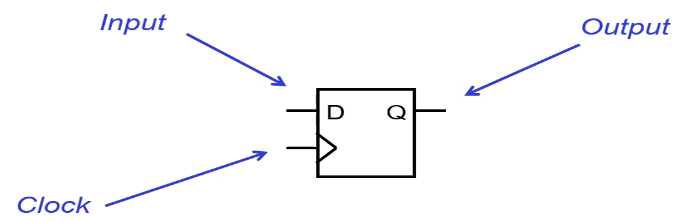
\includegraphics[scale=0.4,frame]{Figures/rtl/D_FF}
\caption{D-FF}
\label{fig:rtl:D_FF}
\end{figure}

\begin{itemize}

\item This type of FF is known as D-FF

\item It has 1 input \verb|D| and 1 clock signal input

\item It has 1 output \verb|Q|

\item Its function: it takes the value of input \verb|D| at the rising edge of the clock, and puts it into \verb|Q|

	\begin{itemize}
	\item Even if the value of \verb|D| changes during the clock period, the value of \verb|Q| stays intact
	
	\item \verb|Q| only changes its value at the next edge of the clock
	\end{itemize}


\end{itemize}


\subsection{Cascading FFs}

Usually in design we cascade FFs as shown in \autoref{fig:rtl:D_FF_cascad}. This causes the signal to propagate through the FFs.

\begin{figure}[h]
\centering
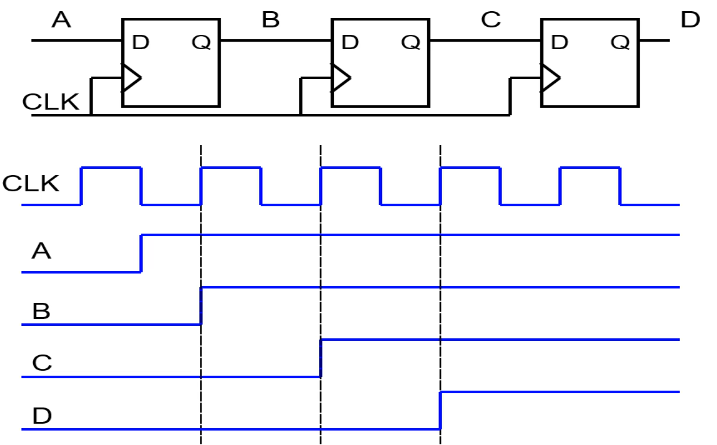
\includegraphics[scale=0.4,frame]{Figures/rtl/D_FF_cascad}
\caption{Cascaded D-FFs}
\label{fig:rtl:D_FF_cascad}
\end{figure}

\begin{itemize}

\item Signal \verb|A| goes high at the $\mathrm{2}^\mathrm{nd}$ rising edge of the clock

	\begin{itemize}
	\item This causes signal \verb|B| to go high
	\end{itemize}

\item The same concept applies between \verb|B| and \verb|C| at the $\mathrm{3}^\mathrm{rd}$ clock cycle

\end{itemize}


\uti{Cascade FF:} \todo{Cascade FF}

\begin{itemize}
\item \textit{I think there is something missing concerning \autoref{fig:rtl:D_FF_cascad}}

\item \textit{I recall that it has something to do with the concept that for D-FF, we need to look at the previous clock period}

\item \textit{I documented this in the HLS report; I will look at it later}

\end{itemize}

\subsection{FFs and Logic}

In a design, we usually add combinational logic in addition to the sequential logic, as shown in \autoref{fig:rtl:D_FF_cascad_comb_logic}.

\begin{figure}[h]
\centering
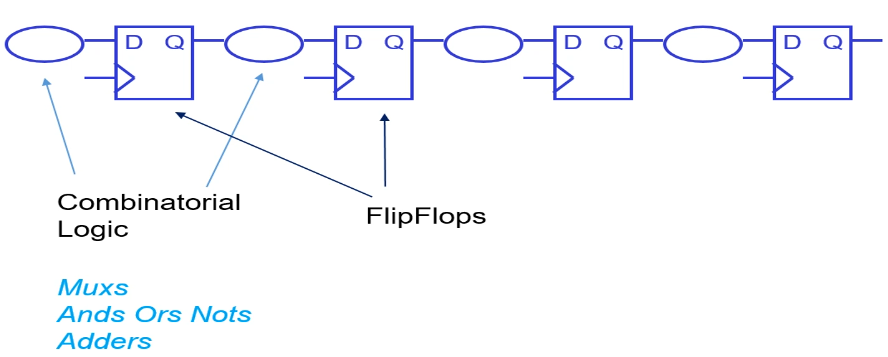
\includegraphics[scale=0.4,frame]{Figures/rtl/D_FF_cascad_comb_logic}
\caption{Cascaded D-FFs with combinational logic}
\label{fig:rtl:D_FF_cascad_comb_logic}
\end{figure}

\begin{itemize}

\item The combinational logic produces an output which is stored in a FF for 1 clock period

\item This output may then be used by the $\mathrm{2}^\mathrm{nd}$ combinational logic before being stored in the $\mathrm{2}^\mathrm{nd}$ FF

\end{itemize}

This is the idea behind what we call RTL design in synchronous design.

\newpage
\subsection{Combinational Delay}

Each time we use combinational logic between FFs, the signal takes some amount of time to propagate from one FF to the next. This is known as the propagation delay.

\begin{figure}[h]
\centering
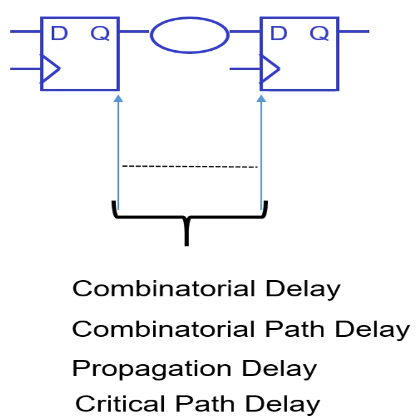
\includegraphics[scale=0.4,frame]{Figures/rtl/comb_prop_delay}
\caption{Propagation delay}
\label{fig:rtl:comb_prop_delay}
\end{figure}

Usually in a design, we have many combinational logic blocks scattered between the FFs, as in \autoref{fig:rtl:critical_delay}. 

\begin{figure}[h]
\centering
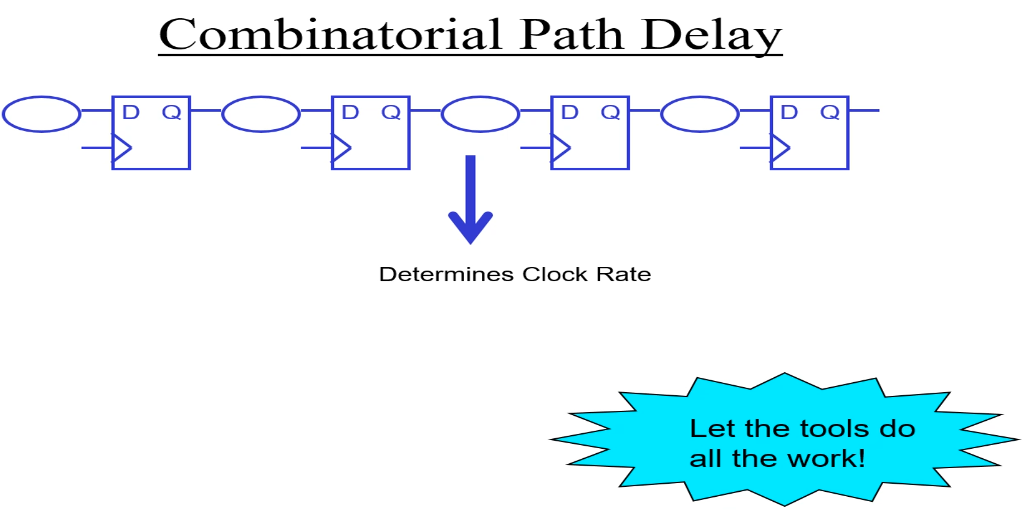
\includegraphics[scale=0.4,frame]{Figures/rtl/critical_delay}
\caption{Critical delay}
\label{fig:rtl:critical_delay}
\end{figure}

What determines the delay of the circuit is the \tbi{combinational circuit with the largest delay}, known as the \tbi{critical delay}.

This is one factor, but we will see later that there are also other factors, and usually we let the place and route tools figure out the delay.\\

\uti{Critical delay} \todo{critical delay}

\begin{itemize}

\item \textit{To review these concepts later in HLS}

\item \textit{Mainly the comparison between propagation delay and clock period, which determines whether or not we use sequential elements}

\end{itemize}


\newpage
\subsection{Metastability}

In every design, there are metastability requirements we need to respect when implementing it.

\begin{figure}[h]
\centering
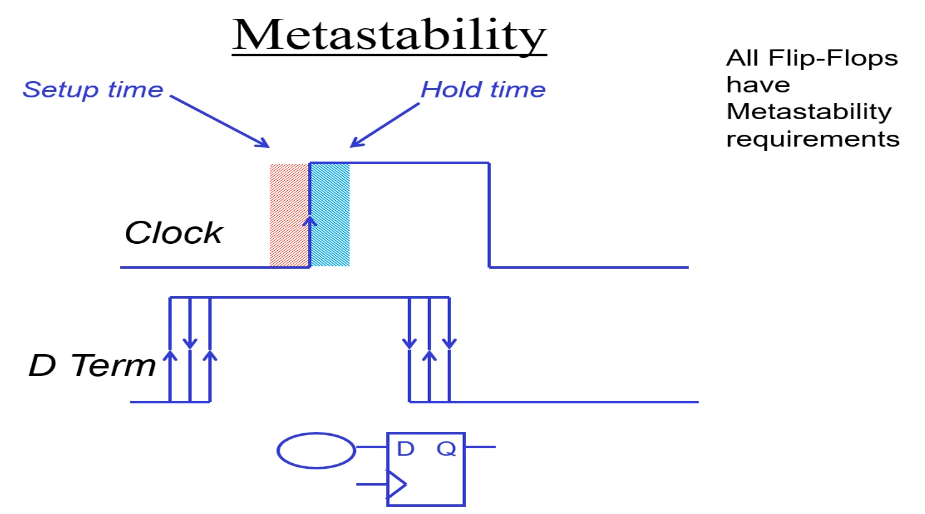
\includegraphics[scale=0.4,frame]{Figures/rtl/metastability}
\caption{Metastability in FPGA}
\label{fig:rtl:metastability}
\end{figure}


\begin{itemize}

\item Setup time: the amount of time \tbi{before rising edge} of the clock where input to FF mush not change

	\begin{itemize}
	\item So as desinger, we should make sure that any combinational logic feeding the \verb|D| input of our FF is stable before the next rising edge of the clock
	\end{itemize}

\item Hold time: same concept of setup time, but it comes \tbi{after the rising edge} of the clock

\end{itemize}

\newpage
How does the metastability seen in \autoref{fig:rtl:metastability} affect our desing ? 

\begin{figure}[h]
\centering
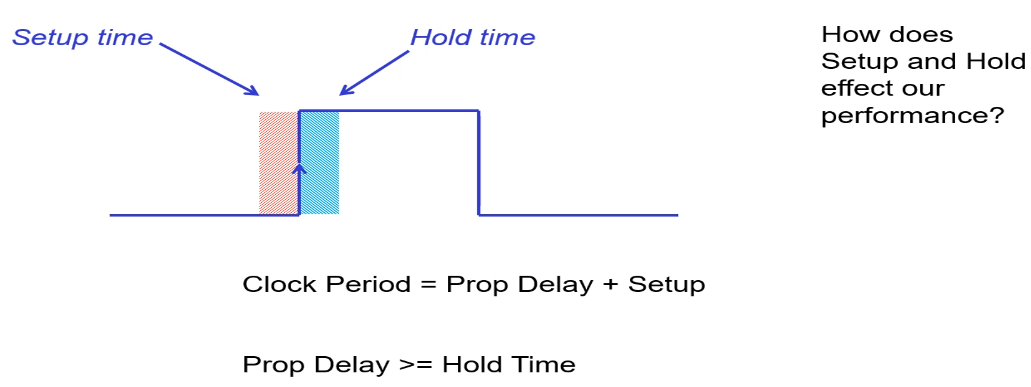
\includegraphics[scale=0.4,frame]{Figures/rtl/metastability_2}
\caption{Metastability effects on performance}
\label{fig:rtl:metastability_2}
\end{figure}

\begin{itemize}

\item It turns out that the clock period lenght will be increased by the amoun of setup time

	\begin{itemize}
	\item That's because the combinatorial result needs to be stable within the setup time requirement prior to the next rising edge of the clock
	\end{itemize}

\item Hold time has opposite effect

	\begin{itemize}
	\item Hold time is met as long as the combinatorial delay is greater than or equal to the hold time.
	\end{itemize}

\end{itemize}

\uti{Hold and setup time:} \todo{Hold and setup time}

\begin{itemize}

\item \textit{I didn't really understand what the author mean in this part concerning the setup and hold time}

\item \textit{To rethink again about these concept, maybe when finishing the chapter and do some exercice}

\end{itemize}


\newpage
\subsection{Clock Skew}

Another concept in desing is known as the clock skew, shown in \autoref{fig:rtl:clk_skew}.

\begin{figure}[h]
\centering
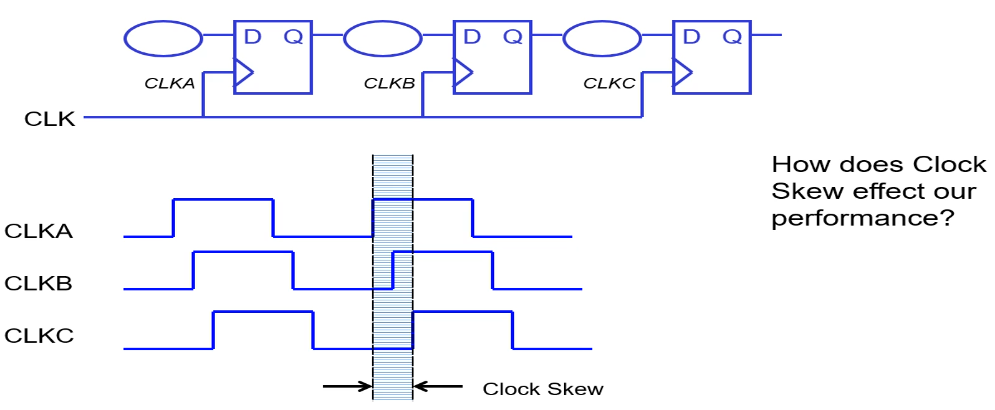
\includegraphics[scale=0.4,frame]{Figures/rtl/clk_skew}
\caption{Clock skew}
\label{fig:rtl:clk_skew}
\end{figure}

Due to the law of physics and electron propagation through the circuit, clock signal arrives at different time at each FF. 
The difference between the last and $\mathrm{1}^\mathrm{st}$ time instant at wich the clock signal arrives is known as \tbi{clock skew}.


This phenomena decrease the clock frequency we can use in an FPGA, and the tools does take care about the compnensation automatically.

\subsection{Clock Domain}

Usually when doing our desing, we apply our clock signal to all our FF in our desing, because tools are good to figure out the desing requirements (setup time, hold time, clock skew,...) for 1 clock domain.


\begin{figure}[h]
\centering
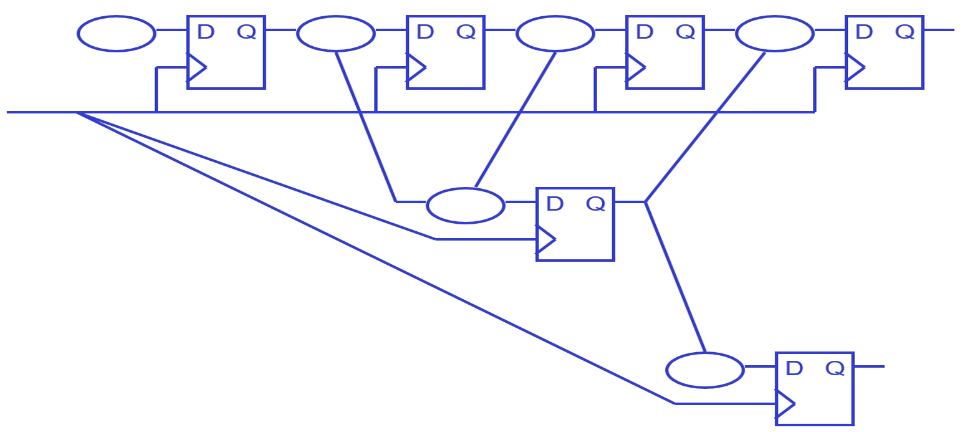
\includegraphics[scale=0.4,frame]{Figures/rtl/clk_domain_single}
\caption{Single clock domain: feeding same clock to all components}
\label{fig:rtl:clk_domain_single}
\end{figure}

\newpage
However, most real desing use multiple clocks, as shown in \autoref{fig:rtl:clk_multi_domain_1}, and this require synchronisation between the data accross the domains

\begin{figure}[h]
\centering
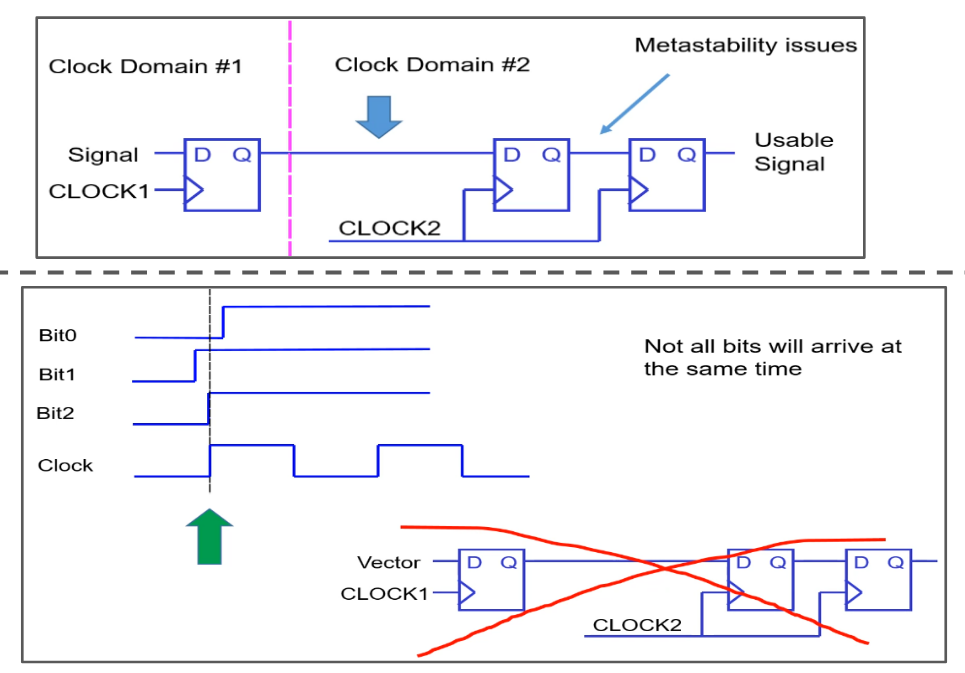
\includegraphics[scale=0.4,frame]{Figures/rtl/clk_multi_domain_1}
\caption{Multiple clock domain}
\label{fig:rtl:clk_multi_domain_1}
\end{figure}

\begin{itemize}

\item One method if we have a signal data, is to pass the input through 2 FF
	\begin{itemize}
	\item the 2 FF stabilize the input and we can use it the signal from the output of the $\mathrm{2}^\mathrm{nd}$ FF
	\end{itemize}

\item However, this mehtod won't work if we have vector data, since bit vectors can arrive at clock instants where bits are changing, and hence we obtain wrong output values of vectors

\end{itemize}

\newpage
It tunrs out the easiest method to pass data between clock domain is a method called asynchronous FIFO, and its an \verb|IP| block provided by many vendors. This technique will be studied in another chapter.\\

\uti{asynchronous FIFO cite:} \todo{asynchronous FIFO cite}

\begin{itemize}

\item \textit{To cite correspondent chapter later}

\end{itemize}

\begin{figure}[h]
\centering
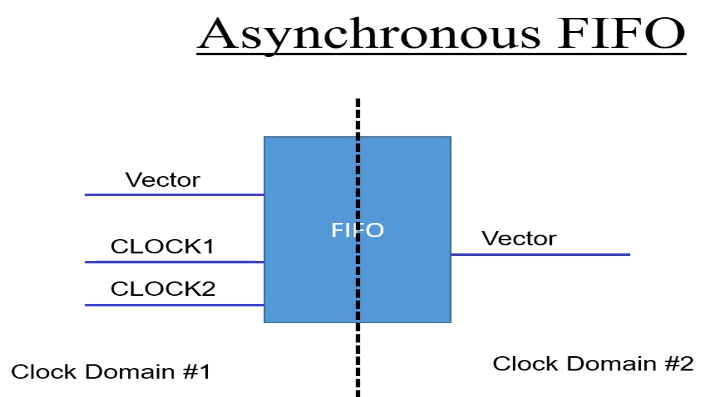
\includegraphics[scale=0.4,frame]{Figures/rtl/async_fifo}
\caption{Asynchronous FIFO}
\label{fig:rtl:async_fifo}
\end{figure}

\newpage
\section{Summary RTL}









